 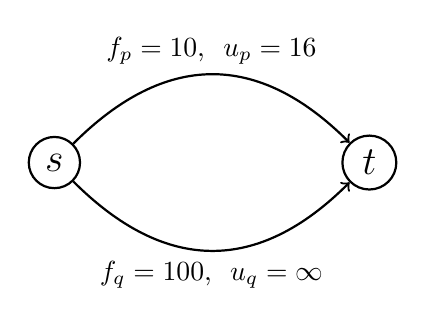
\begin{tikzpicture}[node distance={40mm}, thick, main/.style = {draw, circle}]
    \node[main] (s) {\Large $s$}; 
    \node[main] (t) [right of=s] {\Large $t$};
    \draw[->] (s) to [out=45, in=135, looseness=1.2] node[midway, above] { \green{$f_p = 10$}, \red{ $u_p = 16$}} (t); 
    \draw[->] (s) to [out=-45, in=-135, looseness=1.2] node[midway, below] {\green{$f_q = 100$}, \red{ $u_q = \infty$}} (t); 
\end{tikzpicture} 
